\documentclass[12pt]{report}

\usepackage[a4paper]{geometry}
%\geometry{left=2.5cm,right=2.5cm,top=2.5cm,bottom=2.5cm, a4paper}
\usepackage[utf8]{inputenc}
\usepackage{amsmath}
\usepackage{amsthm}
\usepackage{amssymb}
\usepackage{ulem}
\usepackage{graphicx}
\usepackage{caption}
\graphicspath{}
\usepackage[document]{ragged2e}
\usepackage{setspace}
\usepackage{tabularx}
\usepackage[slovene]{babel}
\usepackage{gensymb}
\usepackage{siunitx}
\usepackage{pdfrender,xcolor}
\usepackage{hyperref}
\usepackage{xurl}
\usepackage{float}
\usepackage{titlesec}

\newfloat{slika}{htbp}{loc}
\floatname{slika}{Slika}

\newfloat{tabela}{htbp}{loc}
\floatname{tabela}{Tabela}

\title{
  
\includegraphics[width=0.4\textwidth]{fmf_logo}\\
  {\small Oddelek za fiziko} \\
  {Michelsenov interferometer}\\
  {\small Poročilo pri fizikalnem praktikumu III}\\

}
\date{}
\author{ Kristofer Č. Povšič \\[5 cm]
 \small  Mentor: Jelena Vesić\\
}


\titleformat{\chapter}[hang]{\Huge\bfseries}{\thechapter{. }}{0pt}{\Huge\bfseries}

\setlength\parindent{0pt}

\begin{document}

\setcounter{page}{2}

\maketitle

\chapter*{Uvod}

Michelsenov interferometer je sestavljen iz treh osnovnih elementov: dveh ravnih zrcal in polprepustnega zrcala.

Interferenčno sliko gledamo na zaslonu oz. če imamo manjšo svetlobo intenziteto, lahko gledamo naravnost v interferometer. 

Polprepustno zrcalo P opišemo z amplitudno odbojnostjo r in prepustnostjo t, ki sta v splošnem kompleksni količini; če ni izgub mora veljati 

\begin{equation}
  |r|^2 + |t|^2 = 1
\end{equation}

Končna delna snopa, ki prideta na izhod 2, imata enaki amplitudi, saj se vsak izmed njiju enkrat odbije na polprepustnem zrcalu (in enkrat gre pa skozi). 

Interferenčna slika je najenostavnejša, če na interferometer pošljemo ravno monokromatsko svetlobno valovanje s krožno frekvenco $\omega$, katerega el. polje zapišemo kot $\vec{E} = \vec{E_0}\cos (kl - \omega t)$, pri čemer je $\vec{E_0}$ amplituda, $k = \frac{\omega}{c_0} = \frac{2 \pi}{\lambda}$ valovni vektor, $l = \int_{a}^{b} n(s) \,ds\ $ pa optično pot. 

V praksi se takemu valovanju zelo dobro približamo s kolimiranim laserskim snopom. Električno polje na opazovalnem zaslon $\vec{E_z}$ jo vsota polj delnih snopov: 

\begin{equation}
  \vec{E_z} = \vec{E_1} + \vec{E_2} = \frac{1}{2} \vec{E_0} (\cos (kl_1 - \omega t) + cos(kl_2 - \omega t))
\end{equation}

pri čemer $l_1$ in $l_2$ označujeta optično pot vsakega delnega snopa. Predfaktor $\frac{1}{2}$ pa izhaja iz sklepa, da nimamo izgb in da je končna amplituda ravno polovična, za vsak delni snop. 

Torej enako vstopni amplitudi, ko snopa seštejemo. Fazna razlika: 

\begin{equation}
  \Delta \phi = k(l_1 - l_2)
\end{equation}

je odvisna od razdalj $d_1$ in $d_2$ med polprepustnim zrcalom P in ravnima zrcala $Z_1$ in $Z_2$ ter od debeline in lomnega količnika materialov, ki jih oba snopa svetlobe prečkata na poti (za polprepustno zrcalo želimo simetrično strukturo, ki je v našem primeru v kocko staknjen pas tako 45 \textdegree prizem, v stičišču pa je dielektrični sloj naparjen na eno izmed obeh prizem). Intenziteto svetlobe na opazovalnem zaslonu je sorazmerna: 

\begin{equation}
  I_z \alpha ||\vec{E_z}||^2 = ||\vec{E_1}||^2 + ||\vec{E_2}|| + 2|\langle \vec{E_1}, \vec{E_2} \rangle|
\end{equation}

in tako dobimo rezultat, da je: 

\begin{equation}
  I_z = \frac{1}{2}I_0(1 + \cos \delta \phi)
\end{equation}

pri čemer $I_0$ označuje intenziteto vpadnega snopa. 

$\Delta \phi = N 2 \pi$ je interferenčni maksimum in $\Delta \phi = (2N + 1) \pi$ je interferenčni minimum. 

 Razliko optičnih poti snopov $\Delta l$ in s tem tudi $\Delta \phi$ lahko spreminjamo s pomikanjem ravnega zrcala. Na zaslonu se pojavijo interferenčni maksimumi in minimumi. Vsakokrat, ko se $Z_1$ premakne $\Delta d_1 = \frac{\pi}{h} = \frac{\lambda}{2}$ se optična pot spremeni za $\Delta l_n = 2 d_1 = \lambda$ in $\Delta \phi$ se poveča za $2\pi$, interferenčna slika se ponovi. 

 Michelsenov interferometer ima posebno nastavite, ki ji pravimo ekvidistančno lega ogledal. Takrat je interferometer nastavljen popolnoma simetrično in sta optični poti enaki, torej je $\Delta \phi$ enaka 0 za vse valovne dolžine. To pomeni, da v tej legi dobimo minimume in maksimume za vse barvne komponente. Blizu ekvidistančne lege vidimo tudi interferenco z belo svetlobo, kar je soroden pojav kot interferenca na tanki plasti (npr. oljni madež). 

 Znameni eksperiment je Michelsenov-Morleyev eksperiment, ki je ovrgel hipotezo o obstoju etra. Danes pa se interferometer uporablja za natančno merjenje dolžin in lomnih količnikov. Uporablja se v visoko ločjivi infra-rdeči spektroskopiji, itd. 


\chapter*{Naloga}

\begin{itemize}
  \item Z laserjem naravnaj interferometer ter umeri pomik zrcala Z1 v odvisnosti od nastavitve mikrometrskega vijaka. 
  \item Izmeri lomni količnik zraka v odvisnosti od zračnega tlaka
  \item Poišči ekvidistančno lego interferometra
  \item Izmeri koferenčno dolžino bele svetlobe iz žarnice na volframsko žarilno nitko 
  \item Izmeri valovni dolžini Na dubleta
\end{itemize}


\begingroup
\let\clearpage\relax

\chapter*{Potrebščine}
\begin{itemize}
  \item Michelsonov interferometer 
  \item He-Ne laser z valovno dolžino $\lambda = (632.8 \pm 0.1)nm$
  \item zračna komora z manometrom in zračna tlačilka 
  \item Hg svetilka in volframska žarnica v istem ohišju
  \item Na svetilka
  \item mlečno steklo, difuzor iz belega papirja
\end{itemize}

\chapter*{Navodilo}

\begin{enumerate}
  \item Naravnaj He-Ne laser, da sveti v sredino polprepustnega ogledala in v sredino obeh zrcal. Naravnaj zrcalo Z2, da se dve svetli "lisi" na zatemnjeni steni laboratorija prekrivata in se pojavijo interferenčne proge. Z vrtenjem mikrometrskega vijaka se interferenčna slika izmenično spreminja.  Vsaka izginula proga pomeni, da se je zrcalo Z1 premaknilo za $\frac{\lambda}{2}$. Mikrometrski vijak postavi na približno sredino in ga vrti ter štej, dokler ne izgine najmanj 100 interferenčnih prog. Odčitaj lego na mikrometrski skali in meritev ponovi petkrat. 
  \item Med polprepustno zrcalo P in pomično zrcalo Z1 pritrdi zračno komoro dolžine $(50 \pm 1)mm$. Povišaj tlak v komori na okoli 2 bar. Z zniževanje pritiska se spreminja lomni količnik zraka v komori in s tem tudi optična pot $l_1$ prvega delnega snopa. Štej izginevanje interferenčnih prog v čim širšem intervalu spremembe tlaka. Meritev števila prog v odvisnosti od tlačne razlike ponovi vsaj petkrat. Vsaka izginula proga pomeni, da se je optična pot $l_1$ spremenila za $\lambda$. Iz znane dolžine celice lahko izračunamo ustrezno spremembo lomnega količnik zraka $\Delta n$ kot funkcijo tlaka. Kolikšen bi bil lomni količnik zraka pri 1000 bar? Ali je primerljiv z lomnim količnikom vode?
  \item Laser zamenjamo z belim svetilom in iščemo lego na mikrometrskem vijaku, pri kateri opazimo interferenčne proge z največji kontrastom. 
  \item Koherenčno dolžino za belo svetlobo ocenimo tako, da opazujemo interferenčno sliko in se z vrtenjem vijaka počasi oddaljujemo iz ekvidistančne lege. Pri tem opazimo, da se kontrast interferenčnih prog manjša. Preštejemo število prog, ko kontrast iz masikmalnega pade na polovico. Meritev je subjektivna in tako lahko ocenimo samo red velikosti in ne dejanskega rezultata. 
  \item Pred vhod interferometra postavimo Na svetilko, vmes pa bel list papirja, ki služi za bolj enakomerno osvetlitev. Na svetilka ima v svojem spektru več emisijskih črt, med katerimi sta najizrazitejši črti pri valovni dolžini, ki daje značilno oranžno barvo svetilu. Razlika valovnih dolžin obeh črt je zelo majna, kar povzroči, da v interferometru poleg interferenčnih prog opazimo spreminjanje kontrasta interferenčnih prog. Podobno kot pri nalogi 1. najprej za 100 ponovitev slike izmerimo premik na mikrometrskem vijaku, nato izmerimo še premik na mikrometrskem vijaku med pobleditvami interferenčnih prog. 
\end{enumerate}

\endgroup


\chapter*{Obdelava podatkov}

\section*{Umeritev interferometra}

Odčitane so bili sledeči premiki za 100 izginulih interferenčnih prog: 

\begin{tabela}
  \centering
  \begin{tabular}{|c|c|} \hline
      meritev & $\Delta x$ \\ \hline
      1 & 0.15 \\ \hline
      2 & 0.16 \\ \hline
      3 & 0.16 \\ \hline
      4 & 0.16 \\ \hline
      5 & 0.17 \\ \hline
  \end{tabular}
\end{tabela}

Izračunam povprečen premik $x = (0.16\pm0.1)mm$. Podatek vstavimo v enačbo: 

\begin{equation}
  R = \frac{N \lambda}{2 x}
\end{equation}

kjer je N število prog in $\lambda = (632.8\pm0.1)mm$. Za računanje z napakami sem uporabil tukaj in tudi v nadaljevanju Pythonova knjižnica \verb+unumpy+ in bila je dobljena vrednost $R = 0.20 \pm 0.01$, kar je precej dobro 1:5 razmerje. 

\section*{Odvisnost lomnega količnika zraka od zračnega tlaka}

Odčitana so bila sledeča števila izginulih interferenčnih prog za spremembo tlaka: 

\begin{tabela}
  \centering
  \begin{tabular}{|c|c|}\hline
    $\Delta p$ & N \\ \hline
    0.5 & 21 \\ \hline
    0.8 & 40 \\ \hline
    1.0 & 58 \\ \hline
    1.5 & 75 \\ \hline
    2.0 & 88 \\ \hline
  \end{tabular}
\end{tabela}

Uporabim enačbo: 

\begin{equation}
  \Delta n = \frac{N \lambda}{2 l}
\end{equation}

kjer je $\Delta n$ lomni količnik, N število izginulih interferenčnih prog, $\lambda = 632.8\pm0.1$ ter l dolžina celice. 
Dobim sledeč graf s pomočjo programerskega jezika \verb+Python+: 

\begin{slika}[H]
  \centering
  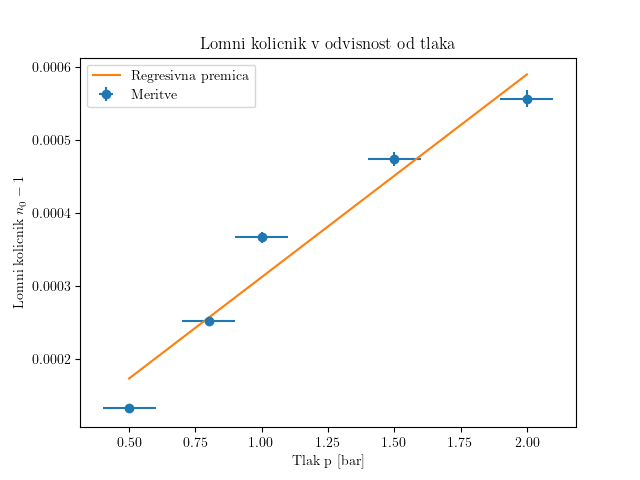
\includegraphics{02}
  \caption{\small Graf odvisnosti lomnega količnika od tlaka}
  \label{fig:graf1}
\end{slika}

Kolikšen bi bil lomni količnik zraka pri 1000 bar? Ali je primerljiv z lomnim količnikom vode?

Če vstavim podatke v enačbo: 

\begin{equation}
  n(p) = n(p_0) + k(p - p_0)
\end{equation}

dobim rezultat $n(1000) = 1.308bar$, kar je primerljivo z lomnim količnikom vode. 

\section*{Ekvidistančna razdalja}

Ekvidistančne nisem uspel najti in so za računske namene naslednjih 2 nalog uporabljeni podatki iz leta 2020, ki so bili posredovani takratnim študentom v sklopu predavanj na daljavo. 

Ekvidistančna razdalja je $d=(6.66 \pm 0.01)mm$. 

\section*{Ocena koherenčne dolžine za belo svetlobo}

Uporabim enačbe: 

\begin{equation}
  d_k = \overline{N}\overline{\lambda}
\end{equation}

kjer je N število prog, $\lambda = 550nm$ in $d_k = (5500 \pm 550)nm$ koherenčna dolžina. 

\begin{equation}
  \tau_k = \frac{d_k}{c}
\end{equation}

 kjer je $\tau_k$ koherenčni čas in c hitrost svetlobe. 

 Vse skupaj vstavim v enačbo:

 \begin{equation}
  \Delta \nu = \frac{1}{\tau_k}
 \end{equation}

 kjer je $\Delta \nu = (5.45 \cdot 10^{13}\pm 5.45\cdot 10^{12})Hz$ spektralna širina svetila. 

 \section*{Določitev valovnih dolžin Na dubleta}

 Uporabljene so bile sledeče vrednosti: 

 \begin{tabela}
  \centering
  \begin{tabular}{|c|c|}\hline
    meritev & $\Delta x$ \\ \hline
    1 & 0.15 \\ \hline
    2 & 0.145 \\ \hline
    3 & 0.15 \\ \hline
  \end{tabular}
\end{tabela}

Povprečen premik je $đ_{100} = (0.148\pm0.01)mm$ in če upoštevamo prestavno razmerje vijaka je to $đ_{100} ' = (0.0296\pm0.0018)mm$. Razdalja med dvema pobleditvama pa je $đ_2 = (0.31\pm0.01)mm$. 
Preko enačbe

\begin{equation}
  \overline{\lambda}= \frac{2đ_{100}'}{100}
\end{equation}

izračunam povprečno valovno dolžino $\overline{\lambda} = (592 \pm 35)nm$, kjer smo upoštevali, da je razlika valovnih dolžin majhna. 

Za izračun razlike valovnih dolžin med dupletoma uporabimo enačbo

\begin{equation}
  \Delta = \frac{\overline{\lambda}^2}{2đ_2'}
\end{equation}

Dobim dve vrednosti: $\lambda_1 = (592.6\pm35)nm$ in $\lambda_2 = (591.4 \pm 35)nm$. 



\end{document}